\documentclass[11pt]{beamer}

% \usepackage[latin1]{inputenc}
\usepackage{natbib}
\usepackage{amssymb}
\usepackage{amsmath}
\usepackage{minibox}
\usepackage{algorithmic}
\usepackage{algorithm}
\usepackage{graphicx,amsmath} 

\usepackage{amsfonts}
\usepackage{amsthm}
\usepackage{graphics, tikz}
\usepackage{subfigure}
\usepackage{setspace}
\usepackage{color}
\usepackage{wrapfig}

% \usetheme{Boadilla}
% \usetheme{Berlin}
% \usetheme{Warsaw}
% \usetheme{AnnArbor}
% \usetheme{Antibes}
% \usetheme{CambridgeUS}
% \usetheme{Copenhagen}
% \usetheme{Darmstadt}
% \usetheme[height=5mm]{Singapore}
\usetheme{Amsterdam}
\usecolortheme{dolphin} 
\usecolortheme[rgb={0,0.17,0.45}]{structure} 

% \usetheme{EastLansing}

\setbeamertemplate{navigation symbols}{}
% \useoutertheme{infolines}

\addtolength{\textwidth}{6mm}

\def\newblock{\hskip .11em plus .33em minus .07em}

\newcommand{\aut}{\mathcal{A}_{\Sigma}}
\newcommand{\lang}[3]{\langle#1,#2,#3\rangle}
\newcommand{\makeimp}[2]{\textbf{\textcolor{#1}{#2}}}
\newtheorem{lem}{Lemma}
\newtheorem{thm}{Theorem}
\newcommand{\vek}[1]{{\bf {#1}}}
\newcommand{\vx}{{\vek{x}}}
\newcommand{\vy}{{\vek{y}}}
\newcommand{\vY}{{\vek{Y}}}
\newcommand{\vX}{{\vek{X}}}
\newcommand{\vv}{{\vek{v}}}
\newcommand{\vz}{{\vek{z}}}
\newcommand{\vtheta}{{\vek{\theta}}}
\newcommand{\vc}{{\vek{c}}}
\newcommand{\vw}{{\vek{w}}}
\newcommand{\vW}{{\vek{W}}}
\newcommand{\vf}{{\vek{f}}}
\newcommand{\vF}{{\vek{F}}}
\newcommand{\vwa}{{\vek{w}_{1\ldots r}}}
\newcommand{\vft}{{\vek{f}}}

\newcommand{\cV}{{\mbox{$\mathcal{V}$}}}
\newcommand{\cE}{{\mbox{$\mathcal{E}$}}}
\newcommand{\cY}{{\mbox{$\mathcal{Y}$}}}
\newcommand{\cX}{{\mbox{$\mathcal{X}$}}}
\newcommand{\cL}{{\mbox{$\mathcal{L}$}}}

\newcommand{\argmax}{{\text{argmax}}}
\newcommand{\argmin}{{\text{argmin}}}
\long\def\ignore#1{}
\long\def\todo#1{{{\bf TODO: } #1\\}}
\newcommand{\pd}[2]{\frac{\partial#1}{\partial#2}}

\newcommand{\indicate}[1]{[\![{#1}]\!]}
\newcommand{\acc}{{a}}
\newcommand{\vh}{{\vek{h}}}
\newcommand{\wt}{{p}}
\newcommand{\TP}{{A}}
\newcommand{\TPb}{{A}}
\newcommand{\estPerf}{{\hat{A}}}
\newcommand{\estURand}{{\hat{A}_R}}


\newcommand{\estSS}{{\mbox{$\hat{\mu}_S$}}}

\newcommand{\oracle}{{\mbox{Oracle}}}
\newcommand{\ham}{{\mbox{Ham}}}
\newcommand{\estSb}{{\mbox{$\hat{\mu}$}}}
%\newcommand{\estURand}{{\hat{A}_R}}
\newcommand{\sqErr}{{\mbox{Err}}}
\newcommand{\estSqErr}{{\mbox{EstErr}}}
\newcommand{\Err}{{\mbox{$\mathcal{E}$}}}
\newcommand{\loss}{{\mbox{$\mathcal{L}$}}}
\newcommand{\var}{{\sigma}}
\newcommand{\estVar}{{\mbox{$\hat{\sigma}$}}}
\newcommand{\nb}{{r}}
\newcommand{\feature}{{\vek{F}}}
\newcommand{\sign}{{\text{sign}}}
\newcommand{\cond}[1]{[\![{#1}]\!]^0_{-\infty}}

\newcommand{\Lp}{{L^1_k}} \newcommand{\Ln}{{L^2_k}}
\newcommand{\posf}{{f}}
\newcommand{\fp}{{{\posf_1}}} \newcommand{\fn}{{{\posf_2}}}
\newcommand{\np}{{{n_1}}} \newcommand{\nn}{{{n_{2}}}}
\newcommand{\minor}{{\text{minor}}} 

\newlength{\wideitemsep}
\setlength{\wideitemsep}{\itemsep}
\addtolength{\wideitemsep}{1pt}
\let\olditem\item
\renewcommand{\item}{\setlength{\itemsep}{\wideitemsep}\olditem}


\title[{\makebox[.45\paperwidth]{Active Evaluation of Classifiers\hfill%
       \insertframenumber/\inserttotalframenumber}}]{Active Accuracy Estimation on Large Datasets}
\author {Namit Katariya, Arun Iyer, Sunita Sarawagi}
\institute{IIT Bombay}
% \date{}

\bibliographystyle{apalike}

\begin{document}
\begin{frame}
\titlepage
\begin{center}
\large{International Conference on Data Mining, 2012} \\ \vspace*{10pt}
\end{center}
\end{frame}

\AtBeginSection[]
{
  \begin{frame}
    \frametitle{Outline}
    \tableofcontents[currentsection]
  \end{frame}
}

%%%%%%%%%%%%%%%%%%%%%%%%%%%%%%%%%%%%%%%%%%%%%%%%%%%%%%%%%%%%%%%%%%%%%%%%%%%%%%%

% Outline (number of slides in parantheses)
% 1. Goal (1)
% 2. Background 
%	i. Motivation (1)
% 	ii. Related work (1)
% 	iii. Our methods (1-2)
% 3. Results (4-5)
% 4. Summary (1)
% 5. Future work (1)
% 6. Backup slides (3-4)
\setbeamercovered{transparent}

\section{Motivation}
\begin{frame}
\frametitle{Motivation}
\pause
\begin{itemize}
\item Many applications rely on output of imperfect classifiers deployed on large datasets \\ 
\begin{itemize}
\item[] \textbf{Examples}: Web page classification, classifying columns of a table to their semantic types
\end{itemize}
\pause
\item \textbf{Common characteristics} 
\begin{itemize}
\item Large and diverse dataset $D$
\item Labeled data $L$ unrepresentative of the entire dataset
\end{itemize}
\pause
\item \textcolor{blue}{Measured accuracy on labeled set $\neq$ True accuracy on data}
\pause
\item Need a method that can converge to the true accuracy
\begin{enumerate}
\item An algorithm that returns a good estimate $(\hat{\mu})$ of true accuracy $(\mu)$ of the classifier
\item \textit{Scalable algorithm} : should work on large datasets where sequential scan not possible \& data accessible only via an index
\end{enumerate} 
\end{itemize}
\end{frame}

\section{Problem Statement}
\begin{frame}
\frametitle{Problem Statement}
\begin{enumerate}
\item \textbf{Accuracy estimation} : Estimate accuracy of a classifier on a large unlabeled dataset based on a \textcolor{blue}{small, possibly unrepresentative, labeled set} and a human labeler \vspace*{5mm}

\item \textbf{Scalable algorithm} : Perform accuracy estimation on unlabeled data so large that it makes \textcolor{blue}{even a single sequential scan impractical} in an interactive setting
\end{enumerate}
\end{frame}

\begin{frame}
\frametitle{A few results...}


\begin{center}
\begin{figure}
\begin{minipage}[b]{0.45\linewidth}
\begin{center}
\includegraphics[width=\hsize]{figs/e1axis.png}
\end{center}
\end{minipage}
\hspace{2mm}
\begin{minipage}[b]{0.45\linewidth}
15\% to 62\% relative reduction in error compared to existing \linebreak approaches\textit{(See Slogistic)} \\ \vspace{1cm}
\end{minipage}
\end{figure}
\hrule
\begin{figure}
\begin{minipage}[b]{0.45\linewidth}
Within 0.5\% of the estimates of methods based on full scan, while sampling (and labeling) just 2.5k instances from indexed unlabeled data \\
\end{minipage}
\hspace{2mm}
\begin{minipage}[b]{0.45\linewidth}
\begin{center}
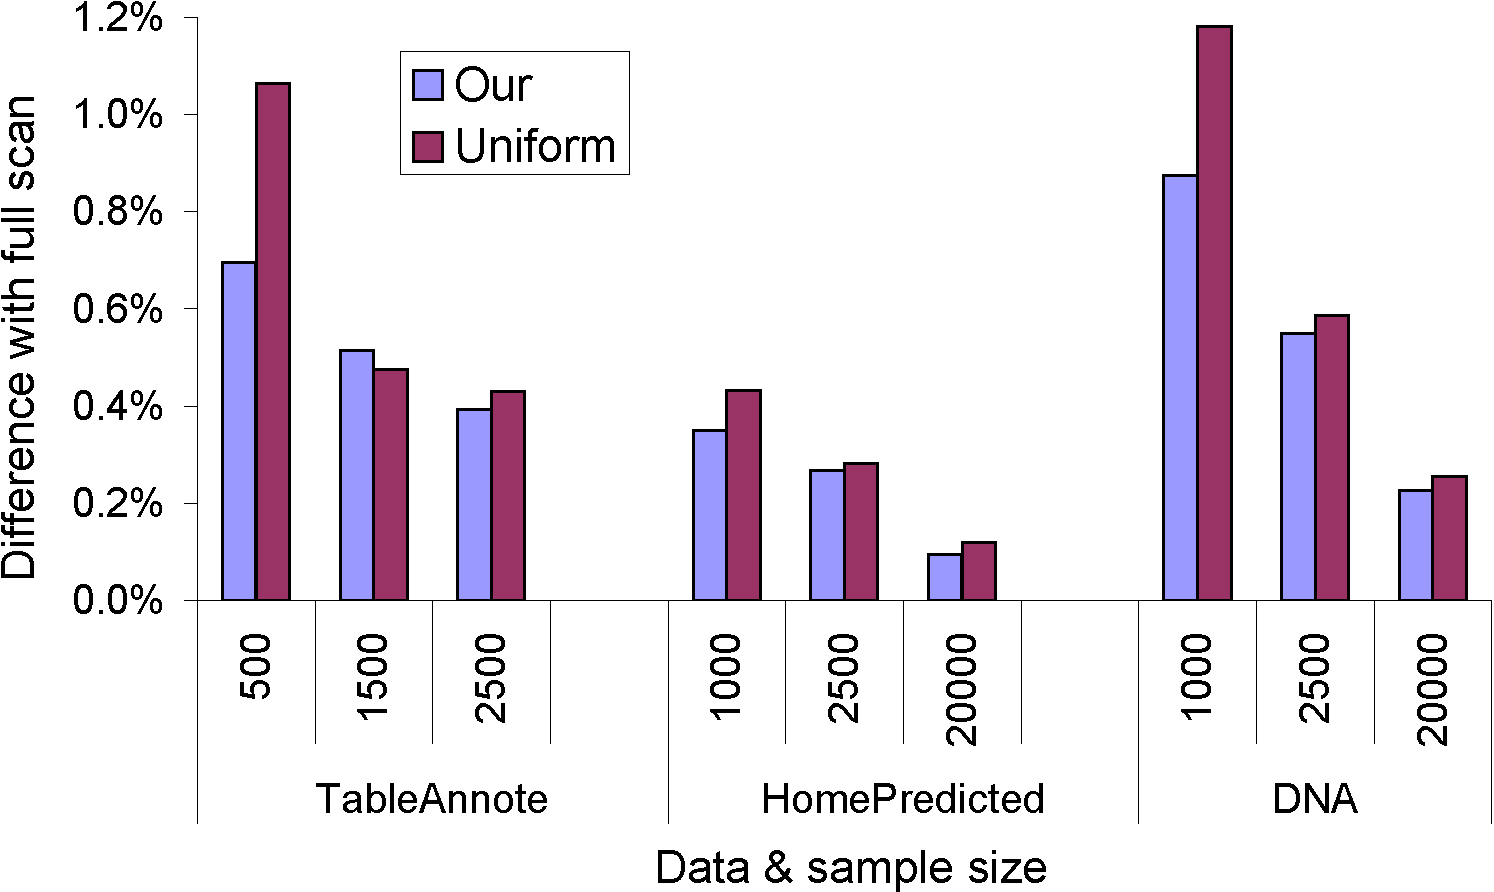
\includegraphics[width=\hsize]{figs/allDataWts-crop}
\caption{\tiny{Comparing methods of sampling from indexed data for
  estimating bucket weights}}
\end{center}  
\end{minipage}
\end{figure}
\end{center}

\end{frame}

\section{Related Work}
\begin{frame}
\frametitle{Related Work}
\begin{itemize}
\pause
\item Most existing work on \textit{learning} rather than \textit{evaluating} classifiers
\pause
\item Existing works on selecting instances for evaluating classifiers:
\begin{itemize}
\item \citep{sawade10} present a new proposal distribution for sampling instances
\item \citep{bennett10} and \citep{druck11} use stratified sampling. However, both assume classifier $C(\vx)$ to be probabilistic and use its $\Pr(y|\vx)$ scores for stratification \& selection
\end{itemize}
\pause
\item Unlike \citep{bennett10} and \citep{druck11}, \textcolor{blue}{instead of fixing the stratification, we learn a new one every time more data gets labeled}
\pause
\item None of the existing methods consider cases where the dataset $D$ is too large to even afford a single sequential scan %Our method is designed to perform accuracy estimation and instance selection on D which can only be accessed via an index.
\end{itemize}
\end{frame}

%%%%%%%%%%%%%%%%%%%%%%%%%%%%%%%%%%%%%%%%%%%%%%%%%%%%%%%%%%%%%%%%%%%%%%

\section{Proposed Solution}
\begin{frame}
\frametitle{Overall Idea}
\begin{algorithm}[H]
\begin{spacing}{0.8}
\begin{algorithmic}[1]\itemsep-5pt
\STATE $B=\text{\#buckets},~\vft=\text{feature vector},~\vwa=\text{hyperplanes}$
\STATE $\estSb_b, \wt_b=\text{accuracy \& weight estimates for bucket b}$
\REPEAT \vspace{5pt}
\STATE Learn stratification function $h(\vft|\vwa)$ 
\STATE Stratify $L$ via $h(.)$ \& compute $\{\estSb_b:1\le b \le B\}$
\STATE Stratify $D$ via $h(.)$ \& compute $\{\wt_b:1\le b \le B\}$
\STATE Display accuracy estimates:  $\estSS=\sum\nolimits_b\wt_b\estSb_b$
\STATE Get stratified sample set $L'$ from $D$
\STATE For each $\vx_i \in L'$, get label $y_i$, and add $(\vx_i,y_i)$ to $L$ \vspace{1pt}
\UNTIL{accuracy $\estSS$ not converged and labeler not bored.}
\STATE{\bf Return} $\estSS$
\end{algorithmic}
\end{spacing}
\caption{Loop for active accuracy estimation}
\end{algorithm}
\end{frame}

\begin{frame}
\frametitle{Learning a stratification strategy} %\vspace{-8mm}
\begin{itemize}
\pause
\item Stratify input space so that instances in each stratum have similar accuracy values
\pause
\begin{itemize}
\item \emph{Supervised clustering methods} : Learn a distance function \\ \textbf{Issue} : Do not scale well 
\item \textbf{Proposal} : Use \textcolor{blue}{Hash codes} based on projections on hyperplanes learned over the feature space
\end{itemize}
\pause
\item Learning hyperplanes (kindly refer to the paper for details)
\begin{itemize}
\item \emph{Smoothing the objective} : Upper-bound with minimum of two convex objectives
\item \emph{Optimizing the smoothed objective} : EM-like algorithm
\item \emph{Ensuring distinct $r$ hyperplanes} : Re-weight instances -- ideas from boosting. 
\end{itemize}
\pause
\item $\estSb_b=\frac{1}{n_b}\sum_{i\in L_b}\acc_i~$ prone to over-fitting. \textcolor{blue}{Smooth based on labeled data in neighbouring buckets}
\pause
\item Method agnostic to the type of classifier under consideration
\end{itemize}
\end{frame}

\begin{frame}
\frametitle{Scaling up -- Instance selection on large amounts of data} 
\begin{itemize}
\pause
\item Unlabeled data accesesed for 
\begin{enumerate}
\item computing $\wt_b=$ the weight corresponding to each bucket $b$ 
\item generating sample $L'$ from $D$ to label and add to $L$
\end{enumerate}
\vspace{1mm}
\pause
%\item \textit{Assumption}: Unlabeled data $D$ indexed so as to partition data into disjoint parts $D_1,\ldots,D_U$. For each partition we can 
%\begin{itemize}
%\item Get its size $N_u$ in terms of number of instances, \& \vspace{-1.5mm}
%\item Generate a uniform random sample of instances within the partition
%\end{itemize}
%\vspace{1mm} \pause
\item Solutions for both, assigning bucket weights and selecting instances, based on sampling from a proposal distribution
\vspace{1mm} \pause
\item In each case, proposal distribution found by setting up an appropriate optimization problem
\pause
\item Optimal proposal distribution can be calculated using some standard assumptions on the index (kindly refer to the paper for details)
\end{itemize}
\end{frame}

%%%%%%%%%%%%%%%%%%%%%%%%%%%%%%%%%%%%%%%%%%%%%%%%%%%%%%%%%%%%%%%%%%%%%%
\section{Results}
\begin{frame}
\frametitle{Results}

\only<1>{
\framesubtitle{Summary of datasets used}
\begin{center}
\begin{table}
\centering
\begin{small}
\begin{tabular}{|l@{}|@{}r|@{}r|@{}r|@{}r|@{}r|}
\hline
Dataset & \multicolumn{1}{c}{\#} \vline & \multicolumn{2}{c}{Size} \vline & \multicolumn{2}{c}{Accuracy (\%)} \vline \\
 & \multicolumn{1}{c}{Features} \vline & \multicolumn{1}{c}{Seed($L$)} \vline & \multicolumn{1}{c}{Unlabeled($D$)} \vline & \multicolumn{1}{r}{Seed($L$)} \vline & \multicolumn{1}{r}{True($D$)} \vline \\
\hline
TableAnnote & 42 & 541 & 11,954,983 & 56.4 & 16.5 \\
Spam & 1000 & 5000 & 350,000 & 86.4 & 93.2 \\
DNA & 800 & 100,000 & 50,000,000 & 72.2 & 77.9 \\
HomeGround & 66 & 514 & 1060 & 50.4 & 32.8 \\
HomePredicted & 66 & 8658 & 13,951,053 & 83.2 & 93.9 \\
\hline
\end{tabular}
\end{small}
\caption{Summary of Datasets}
\end{table}
\end{center}}

\only<2>{
\framesubtitle{Comparison of estimation strategies on the HomeGround dataset}
\begin{center}
\begin{figure}
\includegraphics[width=0.75\hsize]{figs/e1axis.png}
\caption{HomeGround data: Absolute error ($Y$ axis) of different estimation algorithms against increasing number of labeled instances ($X$ axis)}
\end{figure}
\end{center}}

\only<3>{
\framesubtitle{Comparison of estimation strategies on remaining datasets}
\begin{center}
\begin{figure}
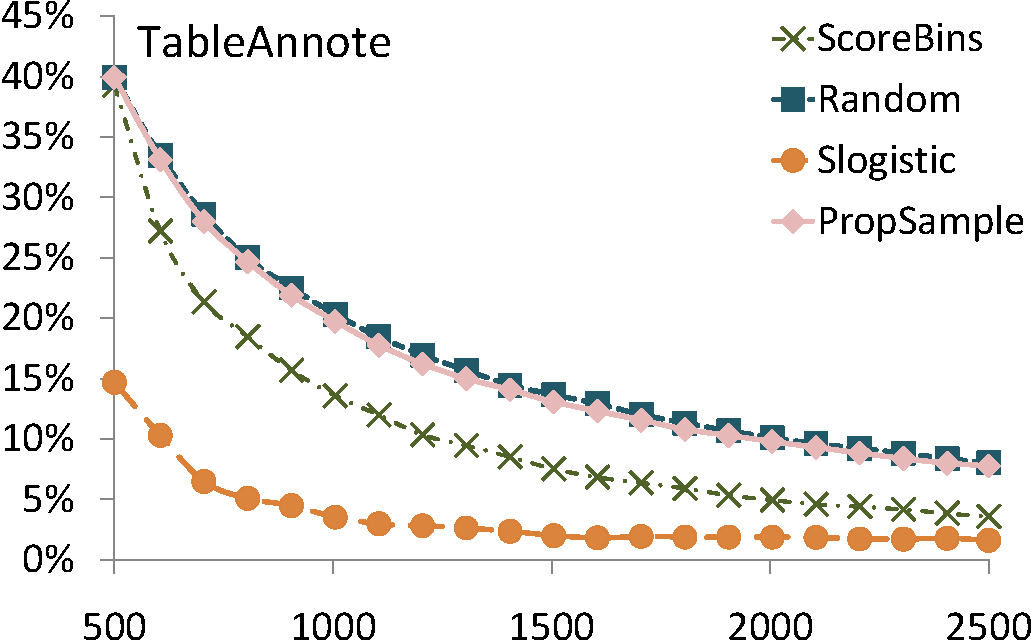
\includegraphics[width=0.37\hsize]{figs/e1tableannote_crop}
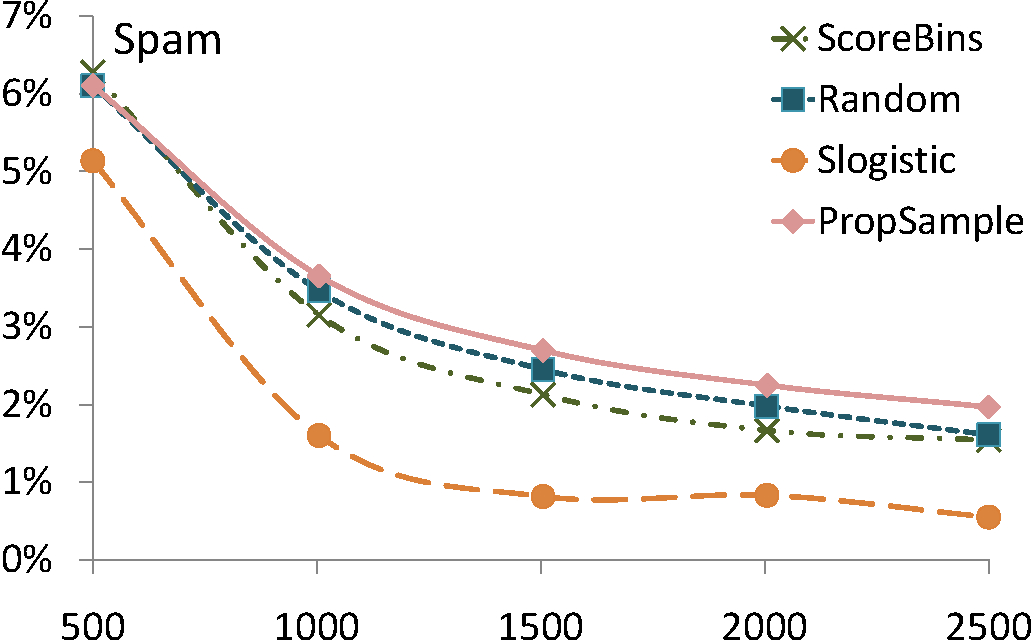
\includegraphics[width=0.37\hsize]{figs/e1spam_crop}
\end{figure}
\begin{figure}
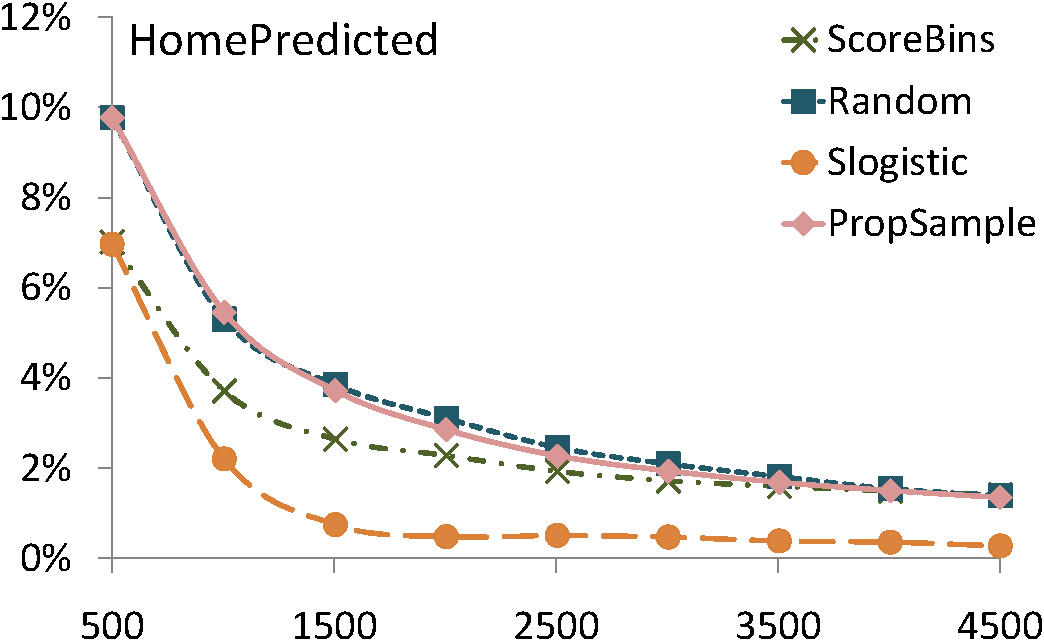
\includegraphics[width=0.37\hsize]{figs/e1homepredicted_crop}
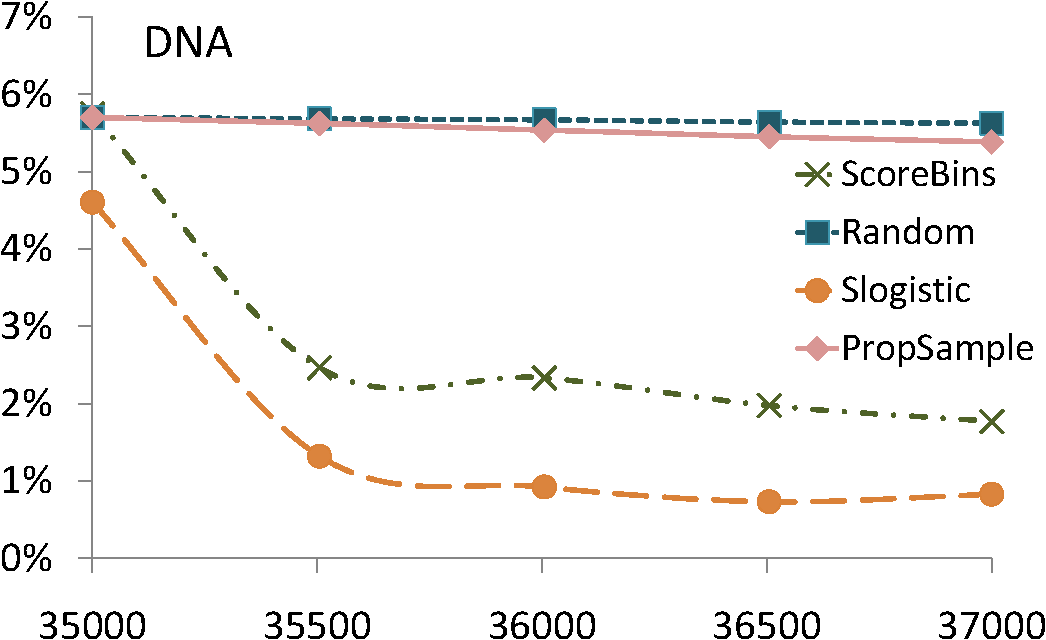
\includegraphics[width=0.37\hsize]{figs/e1dna_crop}
\caption{Absolute error (on the $Y$ axis) of different estimation algorithms against increasing number of labeled instances (on the $X$ axis)}
\end{figure}
\end{center}}

\only<4>{
\framesubtitle{Comparison of different stratification methods on the HomeGround dataset}
\begin{center}
\begin{figure}
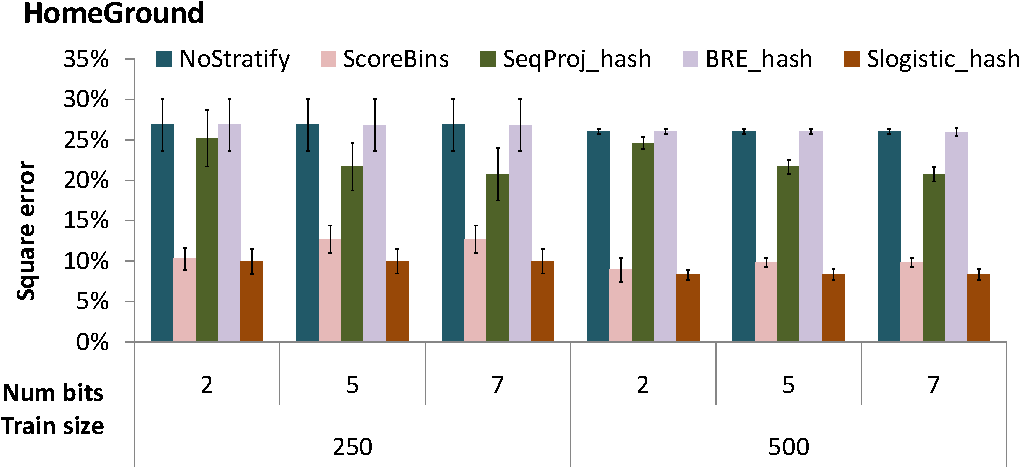
\includegraphics[width=\hsize]{figs/e2homeground_crop}
\caption{HomeGround data: Error of different stratification methods against increasing
  training sizes \& for different number of bits}
\end{figure}
\end{center}}

\only<5>{
\framesubtitle{Comparison of different stratification methods on remaining datasets}
\begin{center}
\begin{figure}
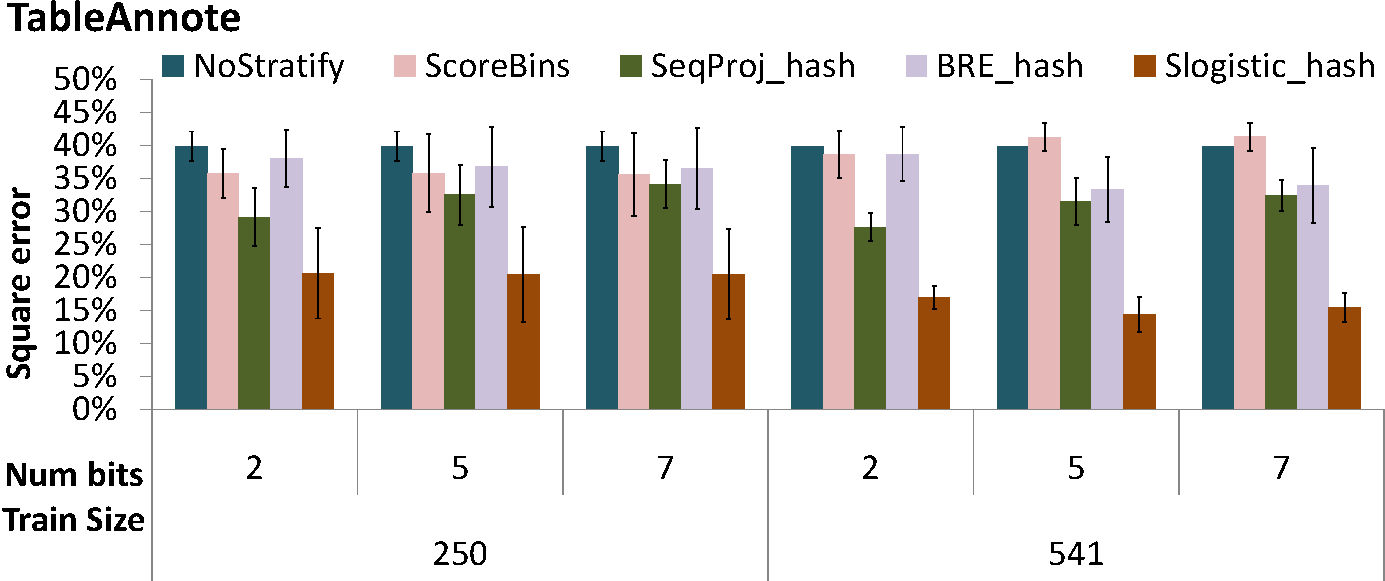
\includegraphics[width=0.5\hsize]{figs/e2tableannote_crop}
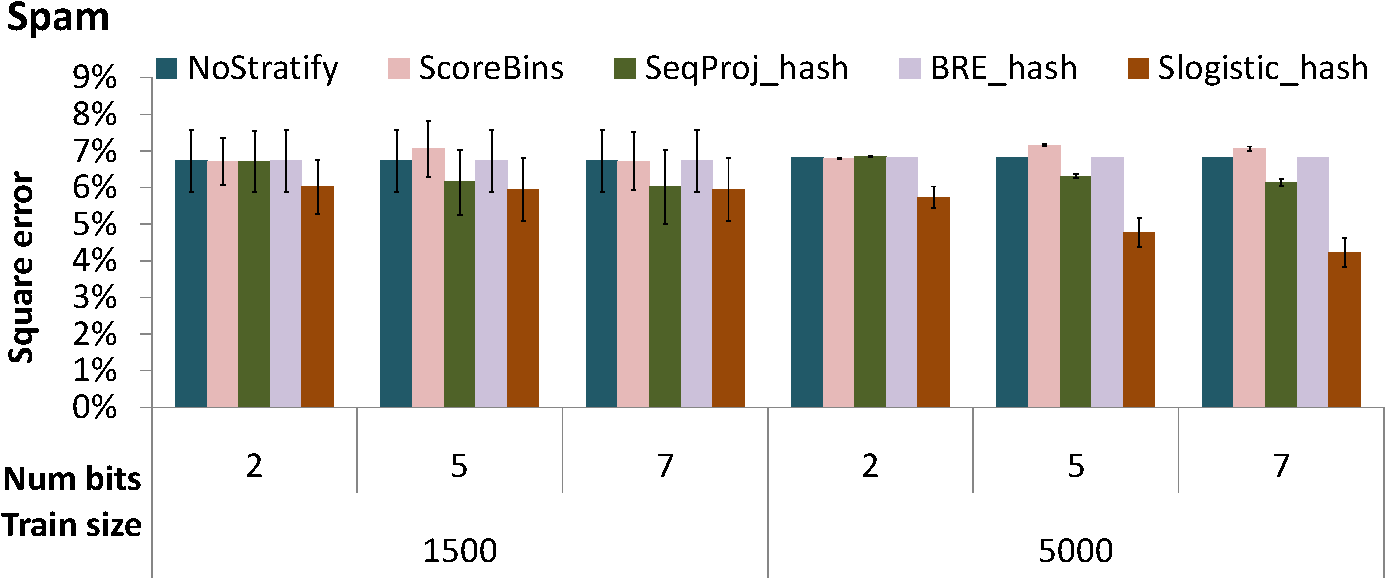
\includegraphics[width=0.5\hsize]{figs/e2spam_crop}
\end{figure}
\begin{figure}
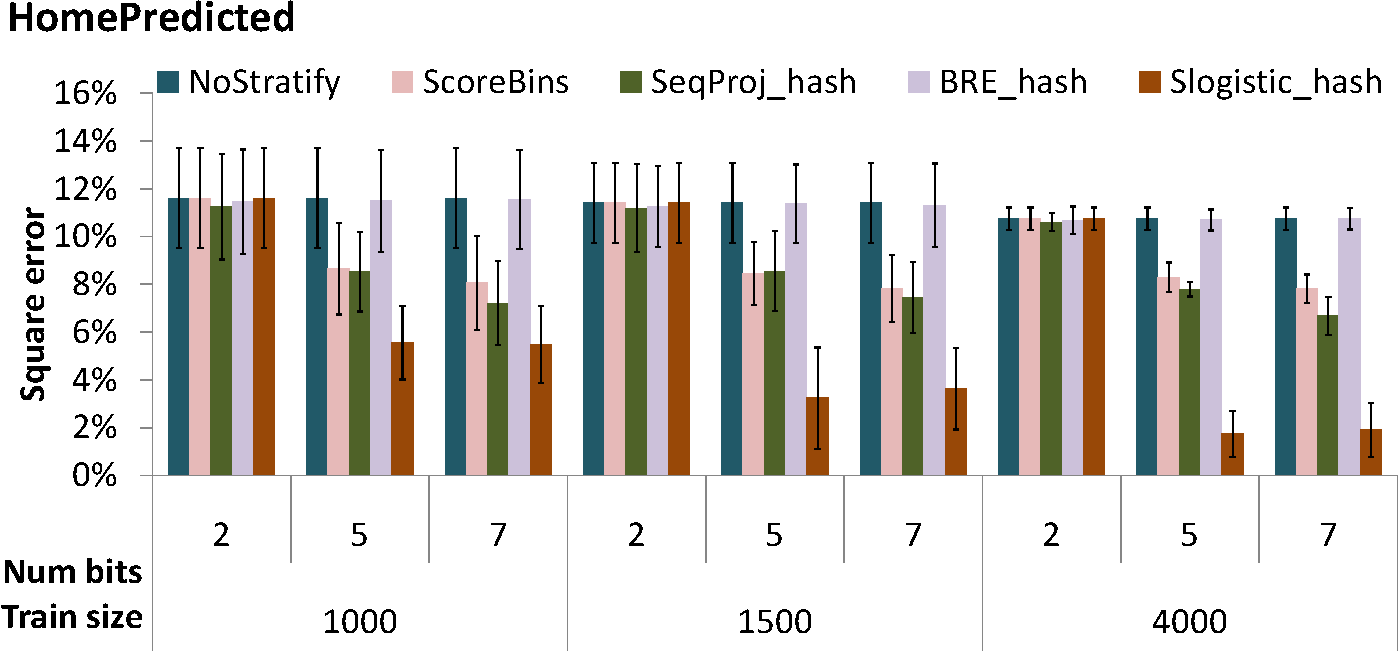
\includegraphics[width=0.5\hsize]{figs/e2homepredicted_crop}
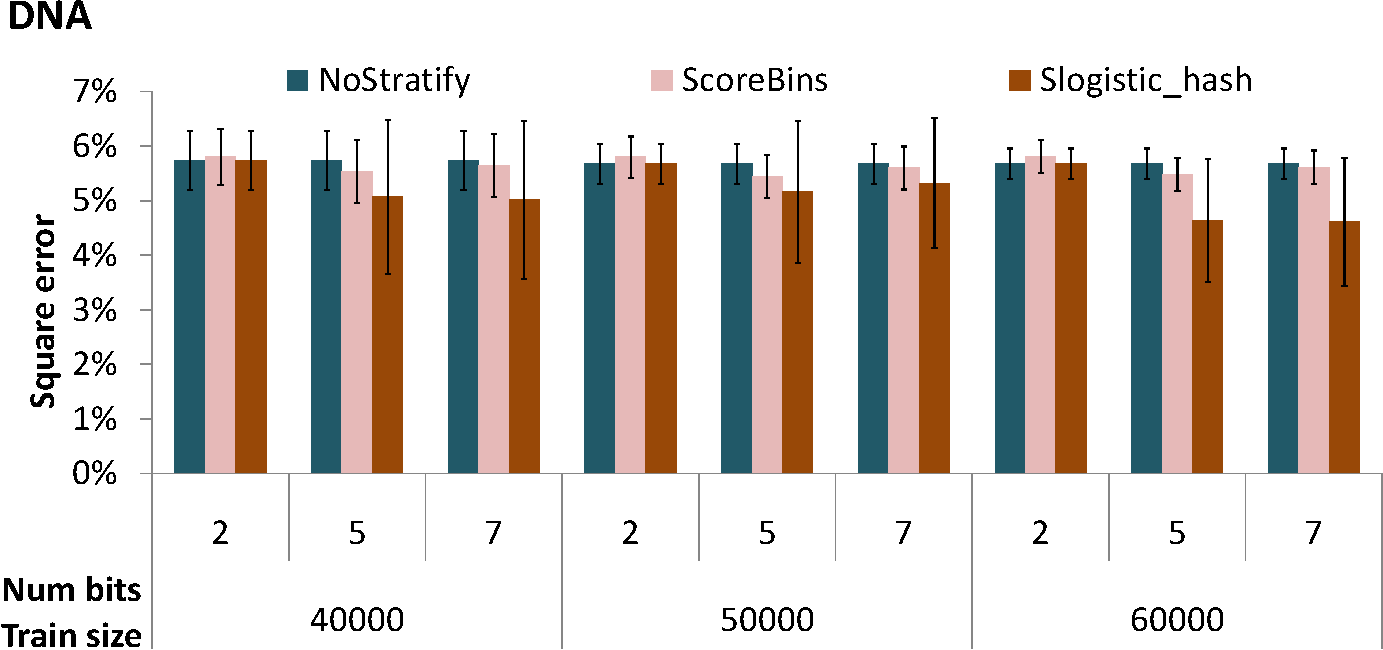
\includegraphics[width=0.5\hsize]{figs/e2dna_crop}
\caption{Error of different stratification methods against increasing
  training sizes and for different number of bits}
\end{figure}
\end{center}}

\only<6>{
\framesubtitle{Comparison of methods of sampling from indexed data for estimating bucket weights}
\begin{figure}
\begin{center}
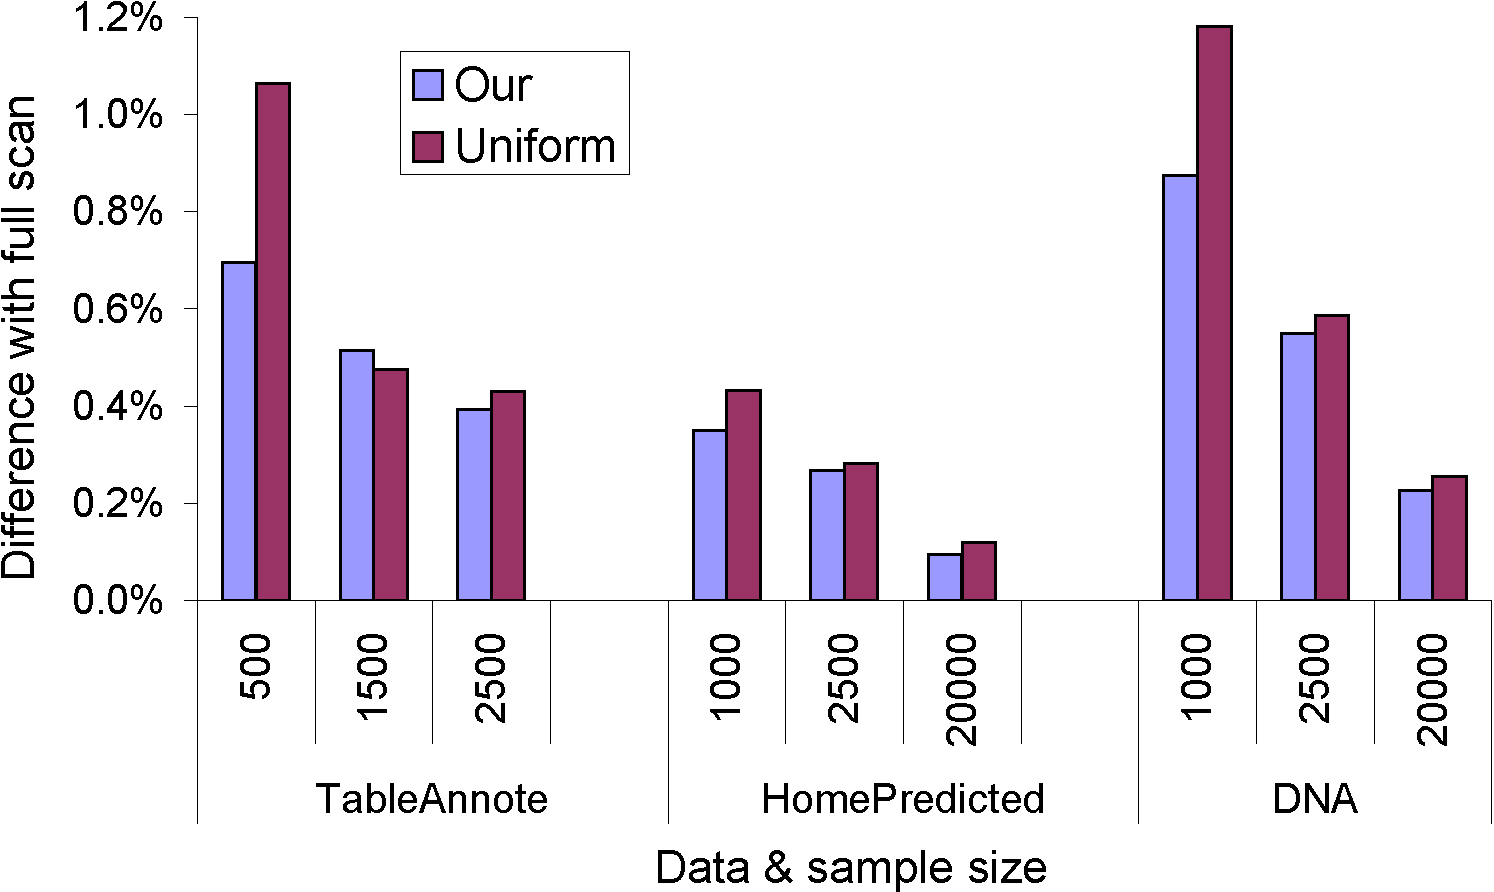
\includegraphics[width=0.85\hsize]{figs/allDataWts-crop}
\caption{Comparing methods of sampling from indexed data for
  estimating bucket weights}
\label{fig:allWts}
\end{center}
\end{figure}}

\end{frame}

%%%%%%%%%%%%%%%%%%%%%%%%%%%%%%%%%%%%%%%%%%%%%%%%%%%%%%%%%%%%%%%%%%%%%%

\section{Summary}
\begin{frame}{Summary}
\begin{enumerate}
\item Addressed the challenge of \emph{\textcolor{blue}{calibrating a classifier's accuracy on large unlabeled datasets} given small amounts of labeled data and a human labeler}
\pause
\item \textcolor{blue}{Proposed a stratified sampling-based method for accuracy estimation} that provides better estimates than simple averaging \& better selection of instances for labeling than random sampling 
\pause
\item Between 15\% and 62\% relative reduction in error achieved compared to existing approaches
\pause
\item Algorithm made \emph{scalable} by proposing \textcolor{blue}{optimal sampling strategies for accessing indexed unlabeled data directly}
\pause
\item Close to optimal performance while reading three orders of magnitude fewer instances on large datasets 
\end{enumerate}
\end{frame}

\begin{frame}
\frametitle{}
\begin{center}
\LARGE{Thank You}
\end{center}
\end{frame}

%%%%%%%%%%%%%%%%%%%%%%%%%%%%%%%%%%%%%%%%%%%%%%%%%%%%%%%%%%%%%%%%%%%%%%

% \section{References}
\begin{frame}[allowframebreaks]{References}
\bibliography{report}
\end{frame}

\begin{frame}
\frametitle{Assigning Bucket Weights}
\begin{itemize}
\item Sample from a proposal distribution : $\hat{\mu}_{S_q} = \frac{1}{|S|}\sum\nolimits_{\vx\in S} \frac{1/N}{q(\vx)}\estSb_{h(\vx)}$
\item \textbf{Result} : When $q(\vx)$ is restricted so that all instances within a partition $u$ are sampled with the same probability $q_u$,
the expected squared error between $\hat{\mu}_{S_q}$ and $\estSS$ is minimized when 
\begin{center} $q_u \propto \sqrt{\sum_{b}\estSb^2_b\wt(b|u)}$ \end{center}
\item $\wt(b|u)$ = fraction of instances in $D_u$ with $h(\vx)=b$
\item Initially, use labeled data to estimate $\wt(b|u)$
\item As more instances are sampled from any $D_u$, refine estimates of $\wt(b|u)$
\end{itemize}
\end{frame}

\begin{frame}
\frametitle{Instance Selection}
\begin{itemize}
\item Perform importance sampling where imp($\vx$) $\propto \estVar_{h(\vx)}$ without evaluating $h(\vx)$ over entire $D$
\item Generate a larger sample $S$ via proposal distribution $q(\vx)$ restricted to choose same $q(\vx) ~\forall \vx$ in data
partition $D_u$ 
\item Then from $S$ generate the sample of $k$ instances by weighting each instance as $f(\vx)/q(\vx)$. Good only if $q(\vx) \sim f(\vx)$
\item Best $q(\vx)$ found by solving for unlabeled bucket weights $q_1,\ldots,q_U$
so that expected L1 distance between $f(\vx)$ and $q(\vx)$ is minimized
\begin{center}
$\min_{q_1,\ldots,q_U} \sum_u\sum_b \wt_u\wt(b|u) \left|\frac{\estVar_b}{Z_f} - q_u\right| ~s.t. \sum_u N\wt_uq_u=1$
\end{center}
\item $Z_f$ approximated as $\sum\nolimits_b\estVar_b\sum\nolimits_u\wt_u\wt(b|u)$
\item Get $\wt(b|u)$ as explained in the previous slide
\end{itemize}
\end{frame}

\end{document}

%%%%%%%%%%%%%%%%%%%%%%%%%%%%%%%%%%%%%%%%%%%%%%%%%%%%%%%%%%%%%%%%%%%%%%%
%
%\section{Sampling on Indexed Data}
%% \subsection{Introduction}
%\begin{frame}
%\frametitle{Sampling on Indexed Data}
%\begin{itemize}
%\item Unlabeled data accessed in 2 different steps of our algorithm
%\begin{itemize}
%\item Calculating fraction $\wt_b$ of instances belonging to each
%bucket $b$; these weights in turn are used to estimate accuracy
%\item When selecting instances for labeling we perform importance sampling where imp($\vx$) $\propto \estVar_{h(\vx)}$. Cannot do a sequential scan over $D$ every time hash function $h(\vx)$ is retrained
%\end{itemize}
%\item \textit{Assumption}: Unlabeled data $D$ indexed so as to partition data into disjoint parts $D_1,\ldots,D_U$. For each
%partition $u$ we can 
%\begin{itemize}
%\item Get its size $N_u$ in terms of number of instances, and 
%\item Generate a uniform random sample of instances within the partition.
%\end{itemize}
%\end{itemize}
%\end{frame}
%
%% \subsection{Assigning bucket weights}
%\begin{frame}
%\frametitle{Assigning Bucket Weights}
%\begin{itemize}
%\item Sample from a proposal distribution : $\hat{A}_{S_q} = \frac{1}{|S|}\sum\nolimits_{\vx\in S} \frac{1/N}{q(\vx)}\estSb_{h(\vx)}$
%\item \textbf{Result} : When $q(\vx)$ is restricted so that all instances within a partition $u$ are sampled with the same probability $q_u$,
%the expected squared error between $\hat{A}_{S_q}$ and $\estSS$ is minimized when 
%\begin{center} $q_u \propto \sqrt{\sum_{b}\estSb^2_b\wt(b|u)}$ \end{center}
%\item $\wt(b|u)$ = fraction of instances in $D_u$ with $h(\vx)=b$
%\item Initially, use labeled data to estimate $\wt(b|u)$
%\item As more instances are sampled from any $D_u$, refine estimates of $\wt(b|u)$
%\end{itemize}
%\end{frame}
%
%% \subsection{Instance Selection}
%\begin{frame}
%\frametitle{Instance Selection}
%\begin{itemize}
%\item Perform importance sampling where imp($\vx$) $\propto \estVar_{h(\vx)}$ without evaluating $h(\vx)$ over entire $D$
%\item Generate a larger sample $S$ via proposal distribution $q(\vx)$ restricted to choose same $q(\vx) ~\forall \vx$ in data
%partition $D_u$ 
%\item Then from $S$ generate the sample of $k$ instances by weighting each instance as $f(\vx)/q(\vx)$. Good only if $q(\vx) \sim f(\vx)$
%\item Best $q(\vx)$ found by solving for unlabeled bucket weights $q_1,\ldots,q_U$
%so that expected L1 distance between $f(\vx)$ and $q(\vx)$ is minimized
%\begin{center}
%$\min_{q_1,\ldots,q_U} \sum_u\sum_b \wt_u\wt(b|u) \left|\frac{\estVar_b}{Z_f} - q_u\right| ~s.t. \sum_u N\wt_uq_u=1$
%\end{center}
%\item $Z_f$ approximated as $\sum\nolimits_b\estVar_b\sum\nolimits_u\wt_u\wt(b|u)$
%\item Get $\wt(b|u)$ as explained in the previous slide
%\end{itemize}
%\end{frame}
%
%%%%%%%%%%%%%%%%%%%%%%%%%%%%%%%%%%%%%%%%%%%%%%%%%%%%%%%%%%%%%%%%%%%%%%%
%
%\section{Experiments}
%% \subsection{Overall Comparison}
%\begin{frame}
%\frametitle{Experiments : Overall Comparison}
%\begin{center}
%\textsc{Error of different estimation algorithms against increasing number of labeled instances} 
%\end{center}
%\begin{center}
%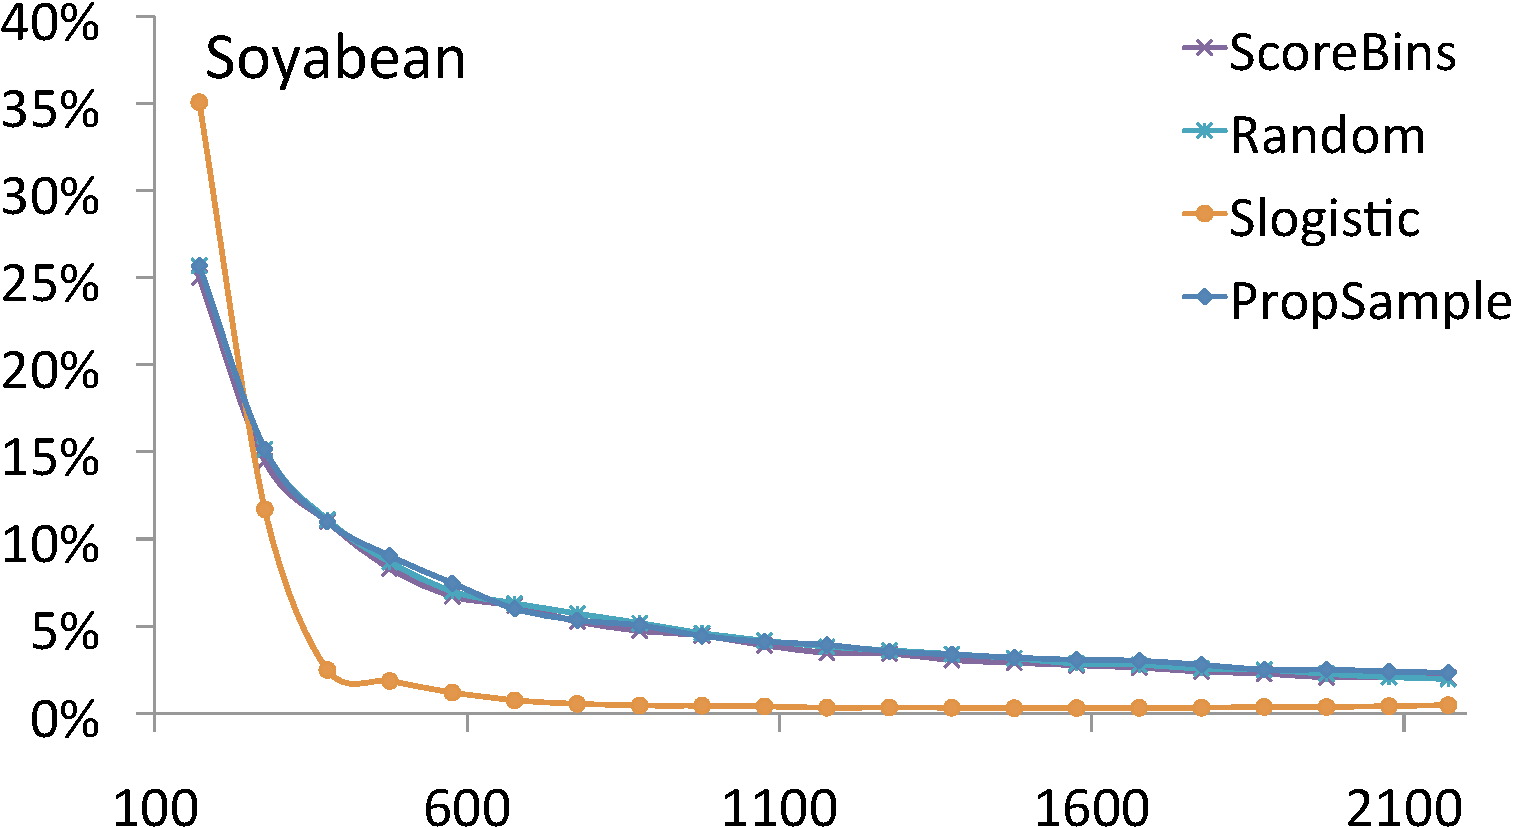
\includegraphics[width=0.34\hsize]{figs/e1wekacrop}
%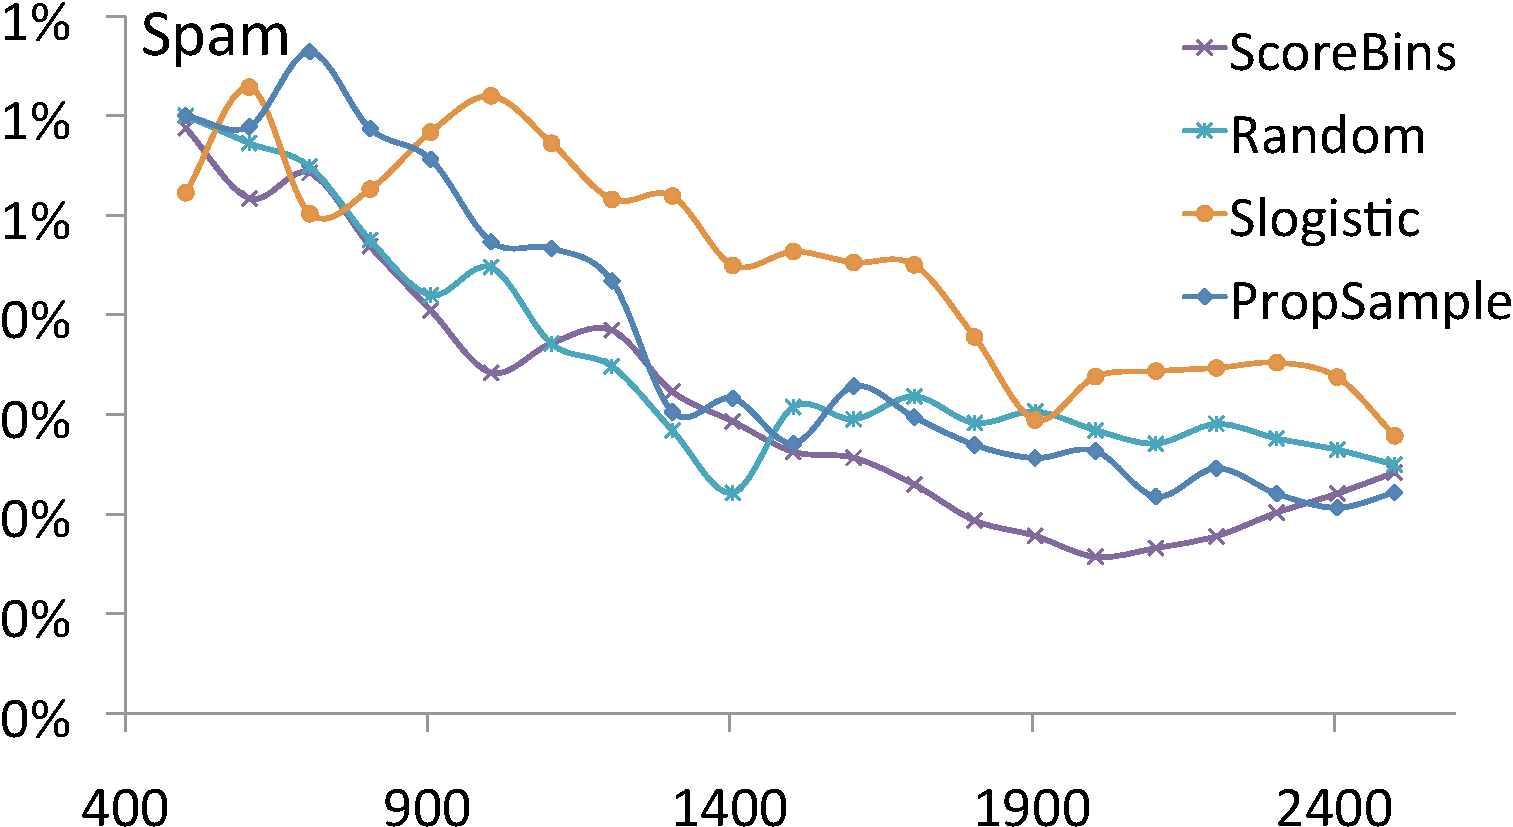
\includegraphics[width=0.34\hsize]{figs/e1webspamcrop}
%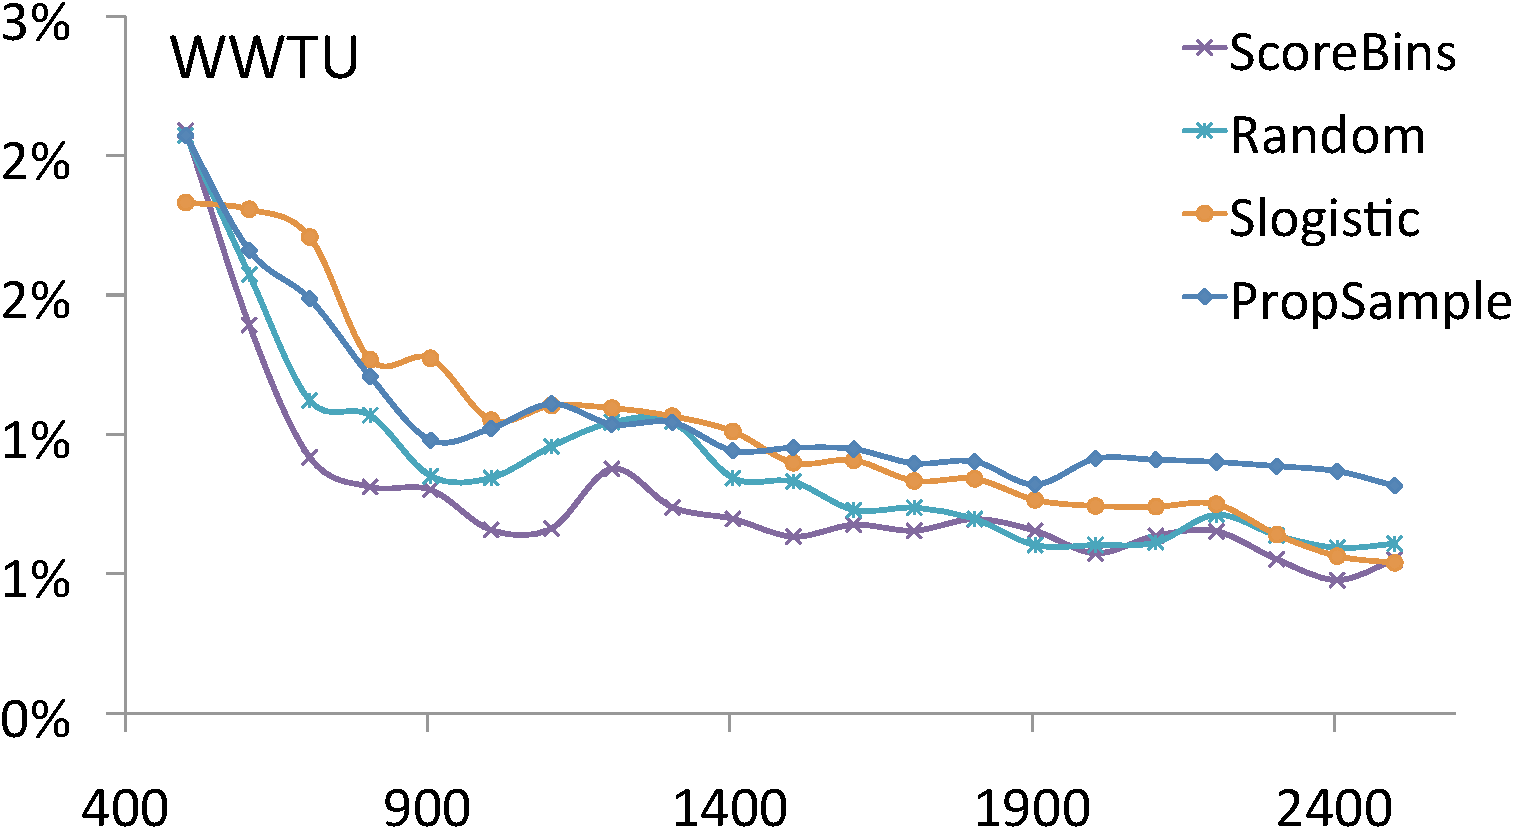
\includegraphics[width=0.34\hsize]{figs/e1wwtucrop}
%\end{center}
%\begin{center}
%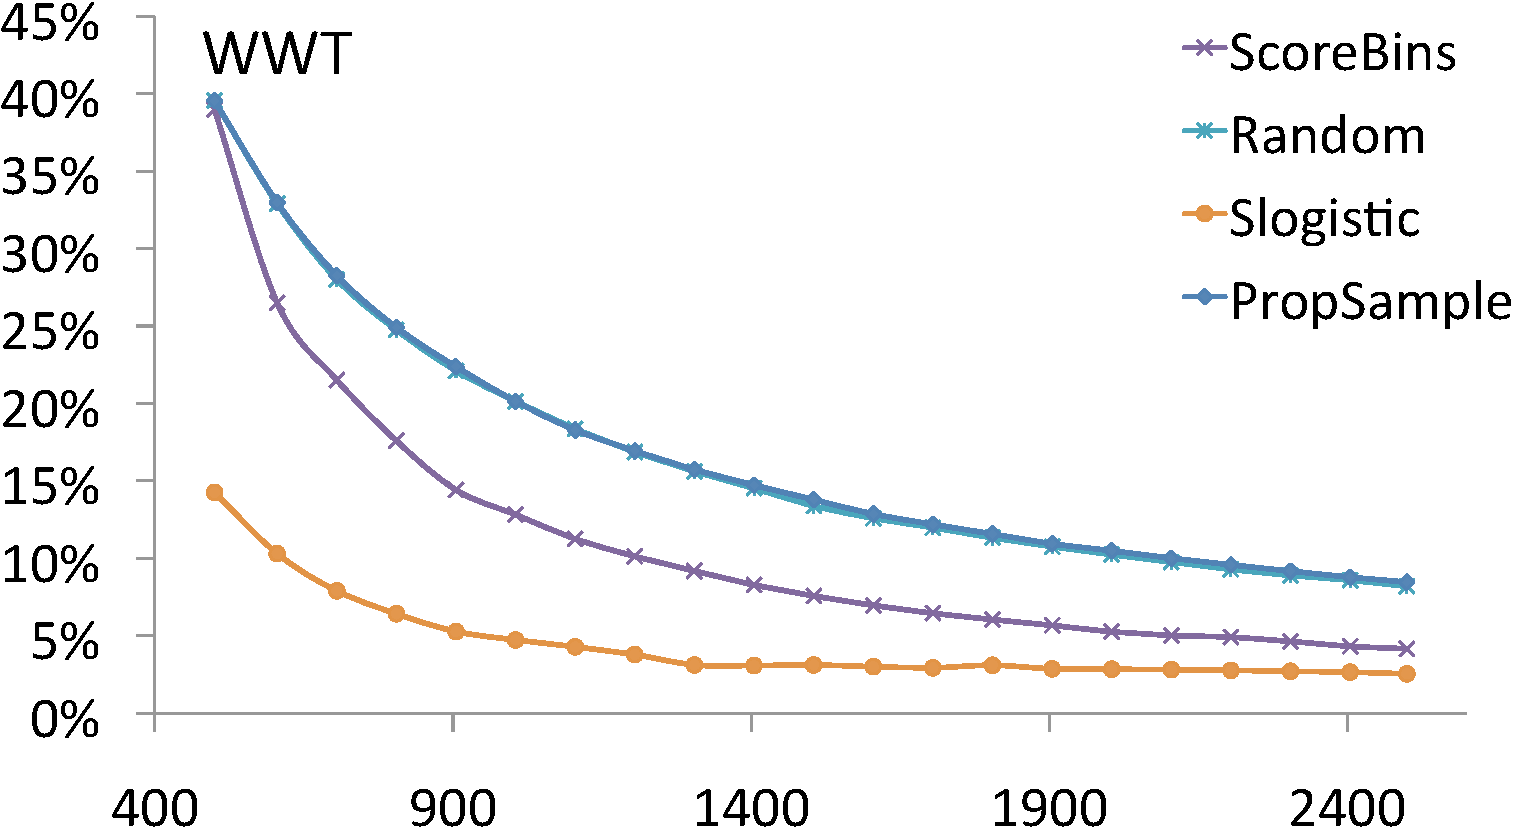
\includegraphics[width=0.35\hsize]{figs/e1wwtcrop}
%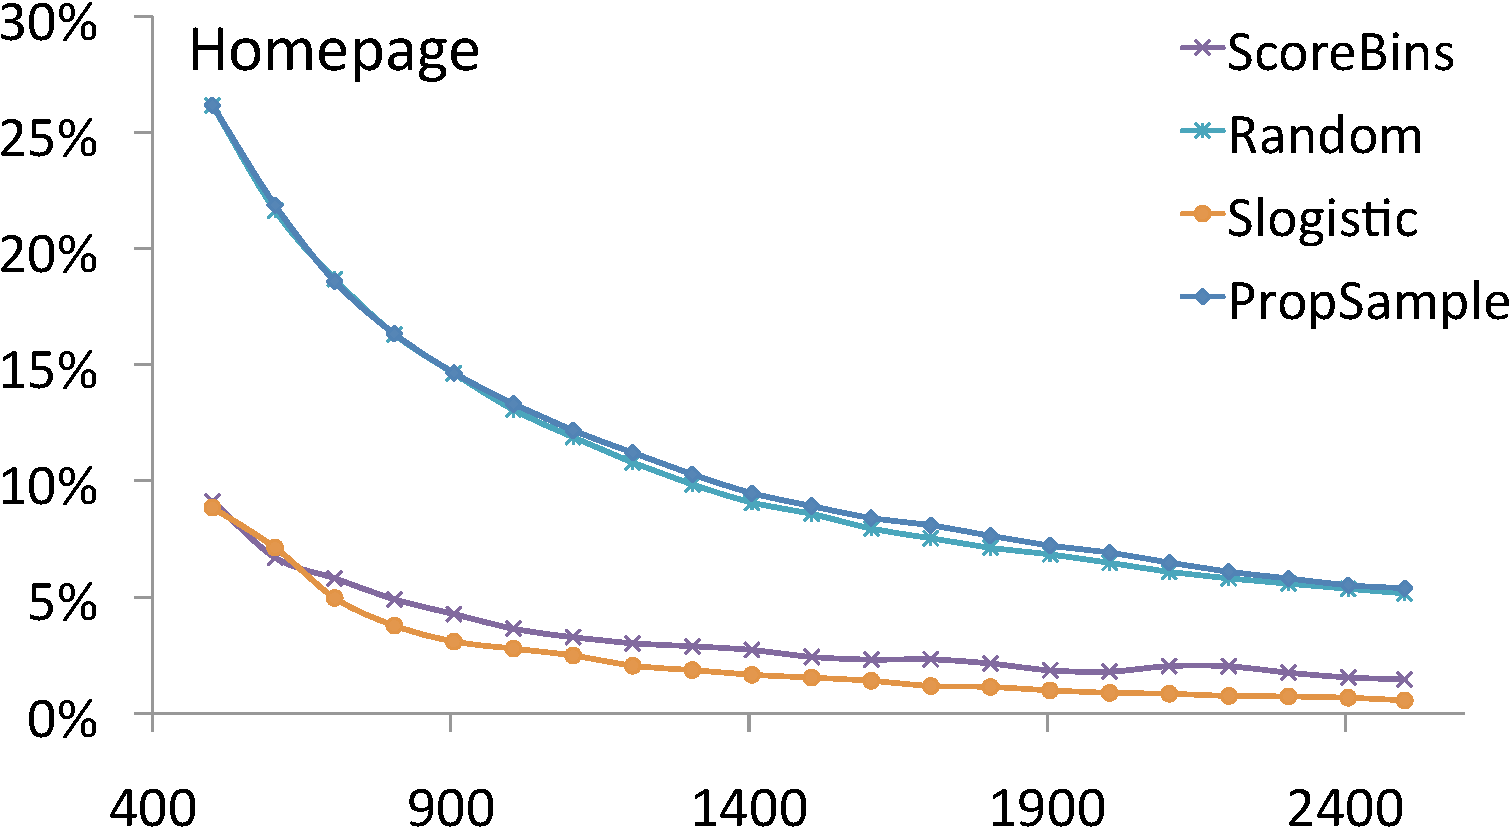
\includegraphics[width=0.35\hsize]{figs/e1ydatasetcrop}
%\end{center}
%\end{frame}
%
%% \subsection{Comparison of Stratification Methods}
%\begin{frame}
%\frametitle{Comaprison of Stratification Methods}
%\begin{center}
%\textsc{Error of different stratification methods against increasing training sizes \& for different no. of bits}
%\end{center}
%\begin{center}
%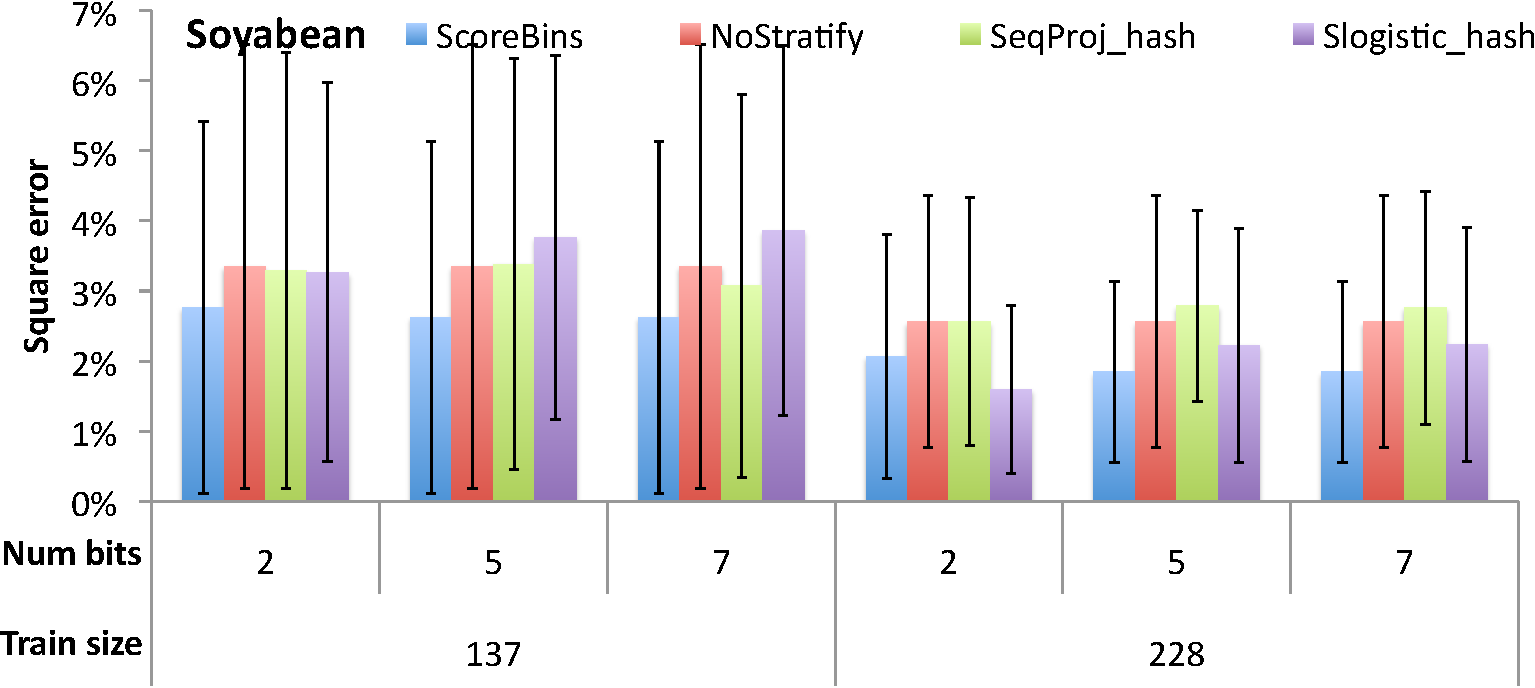
\includegraphics[width=0.34\hsize]{figs/e2wekacrop}
%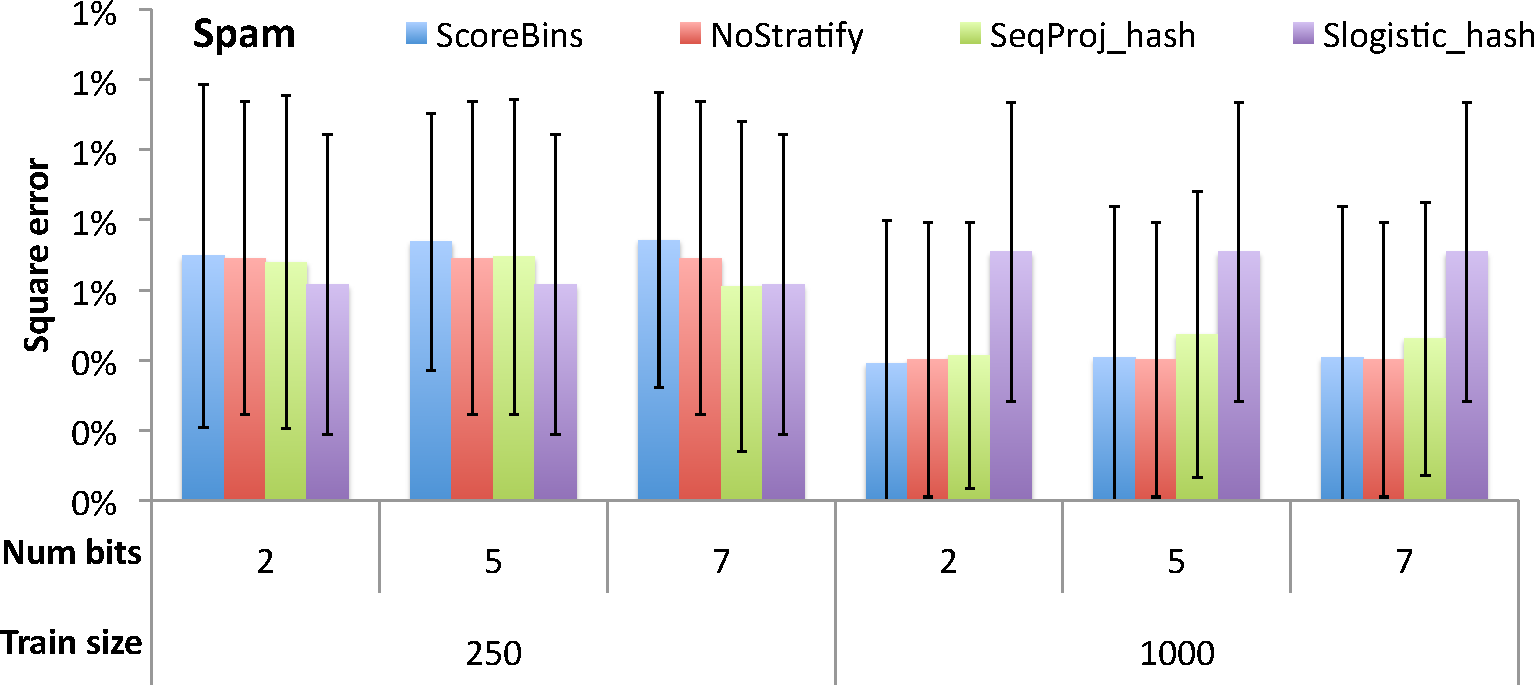
\includegraphics[width=0.34\hsize]{figs/e2webspamcrop}
%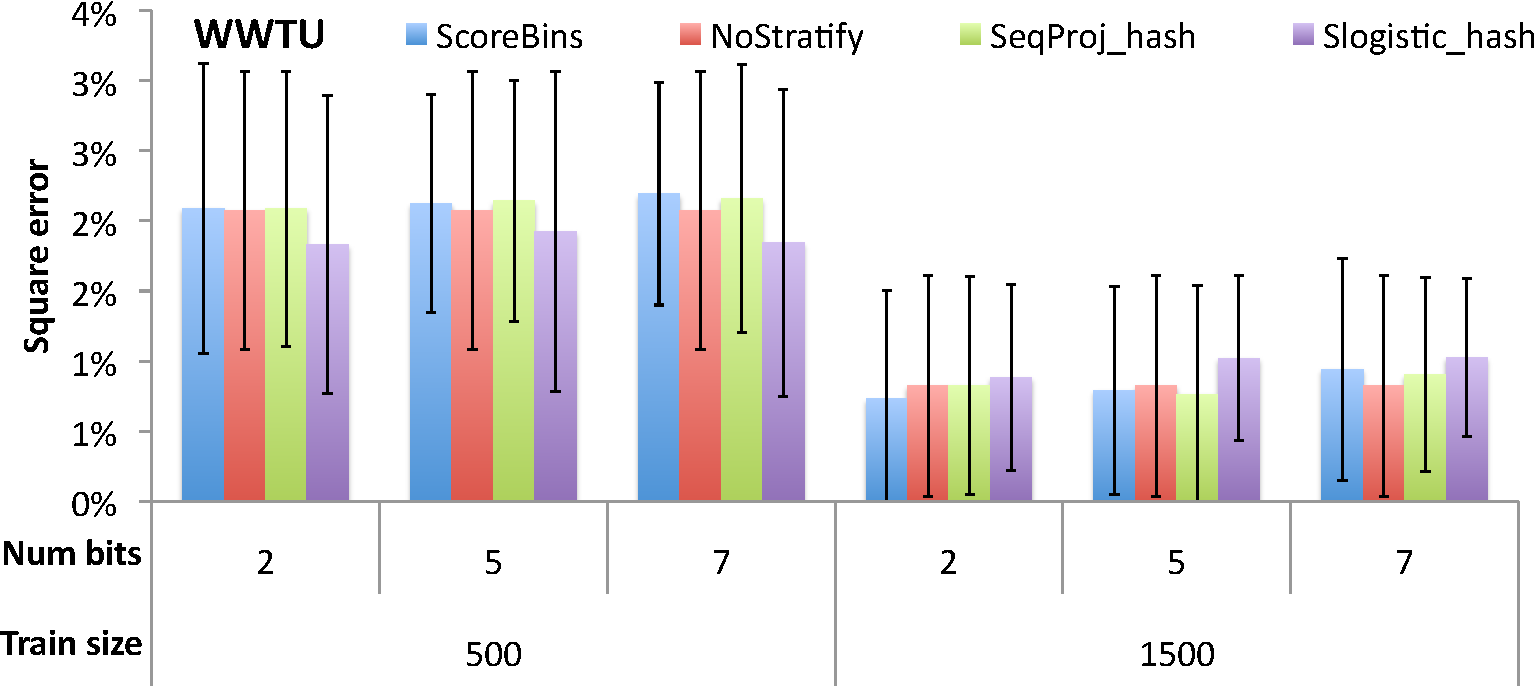
\includegraphics[width=0.34\hsize]{figs/e2wwtucrop}
%\end{center}
%\begin{center}
%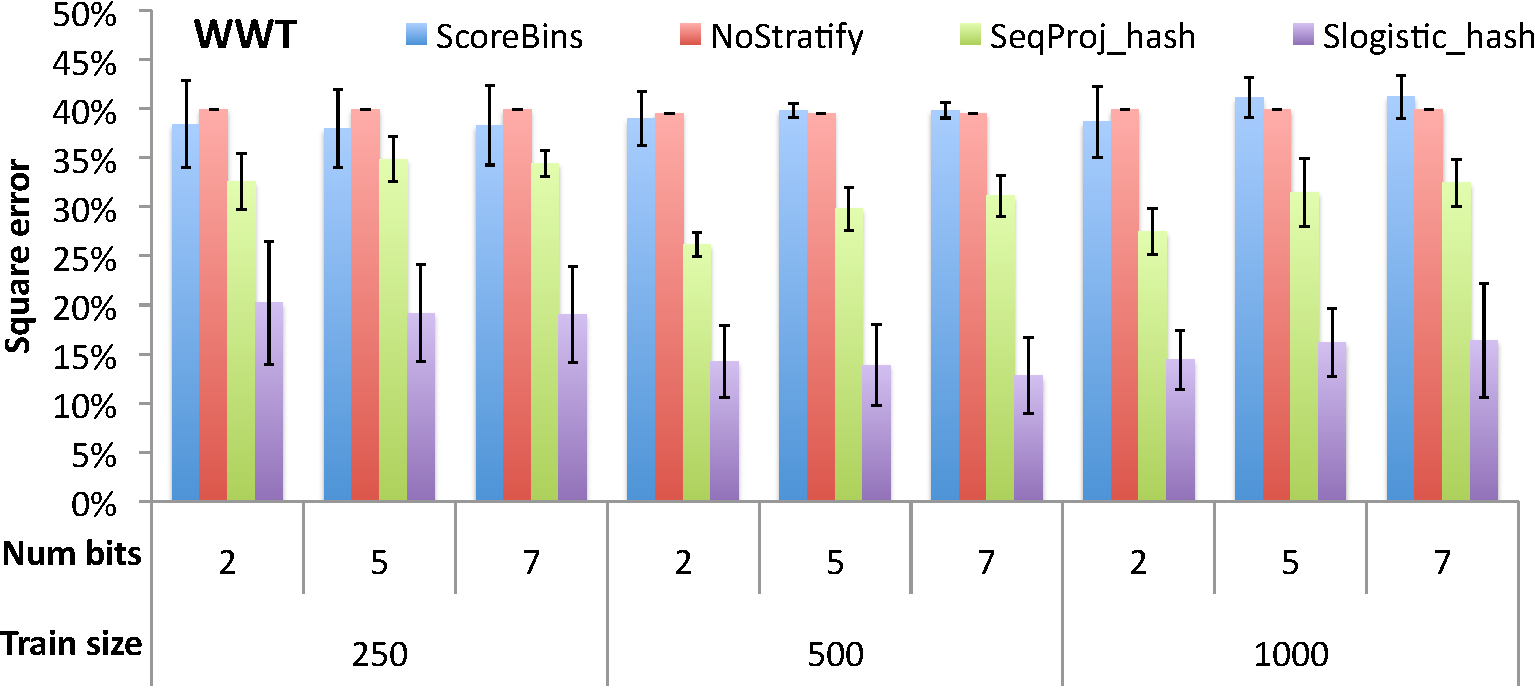
\includegraphics[width=0.42\hsize]{figs/e2wwtcrop}
%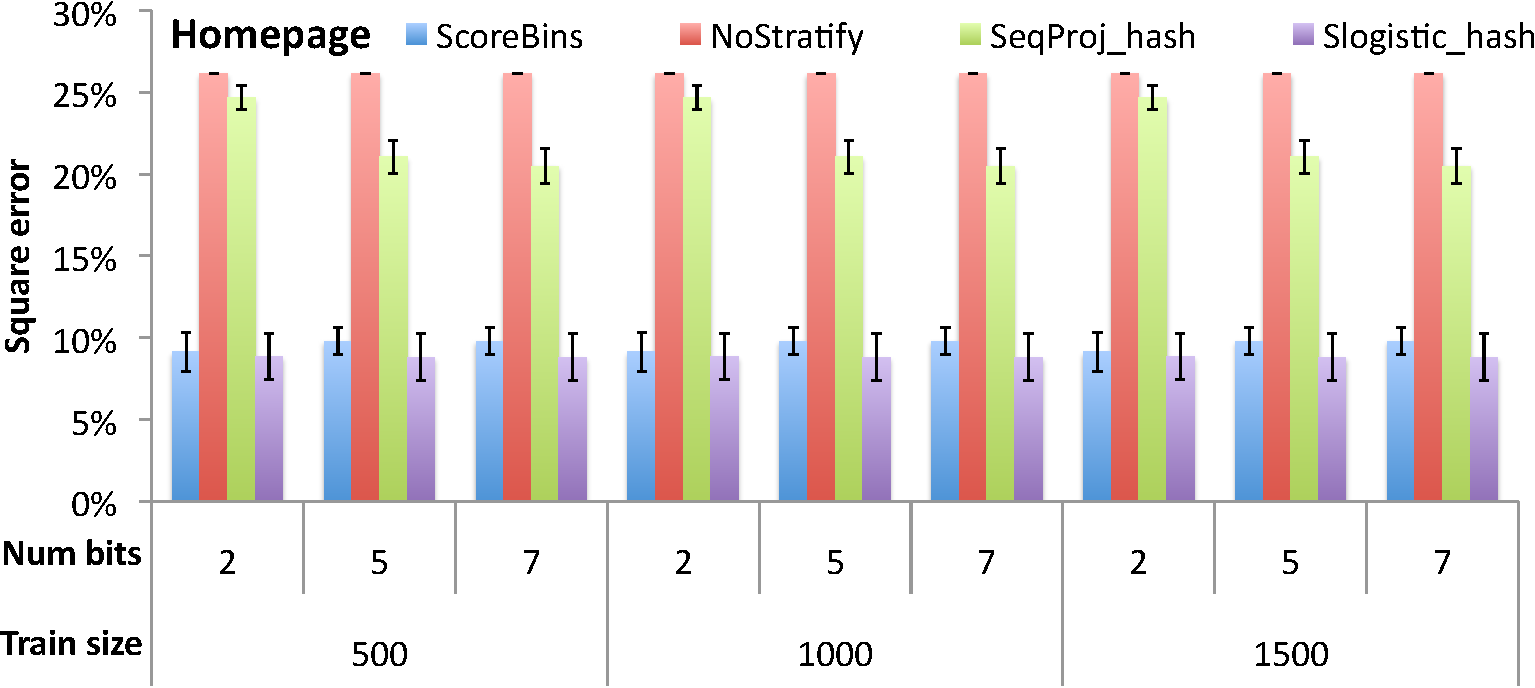
\includegraphics[width=0.42\hsize]{figs/e2ydatasetcrop}
%\end{center}
%\end{frame}
%
%% subsection{Efficiency of Indexed Data Access}
%\begin{frame}
%\frametitle{Efficiency of Indexed Data Access}
%\begin{center}
%\textsc{Comparing methods of sampling from indexed data for estimating bucket weights}
%\end{center}
%\begin{center}
%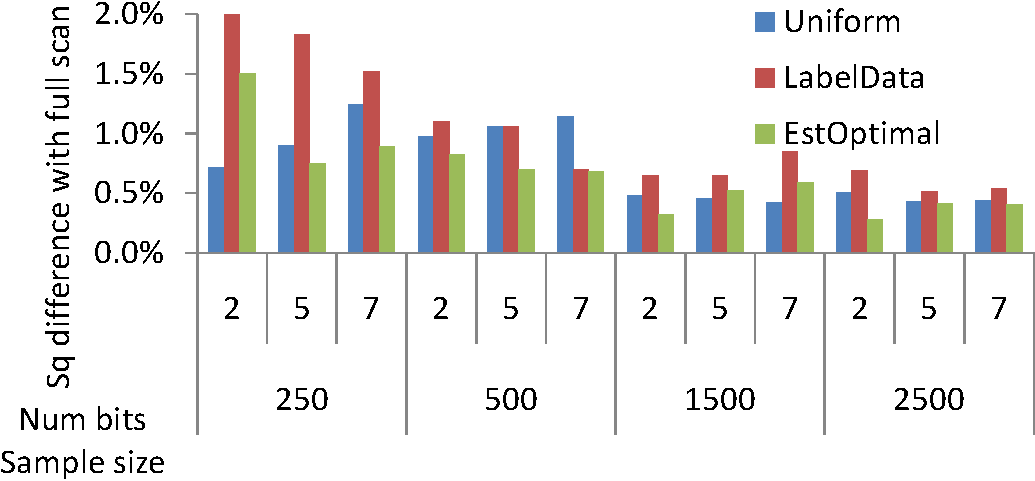
\includegraphics[width=0.45\hsize]{figs/allWts-crop}
%\end{center}
%\begin{center}
%\textsc{Error of different methods for selecting instances for labeling against increasing labeled data}
%\end{center}
%\begin{center}
%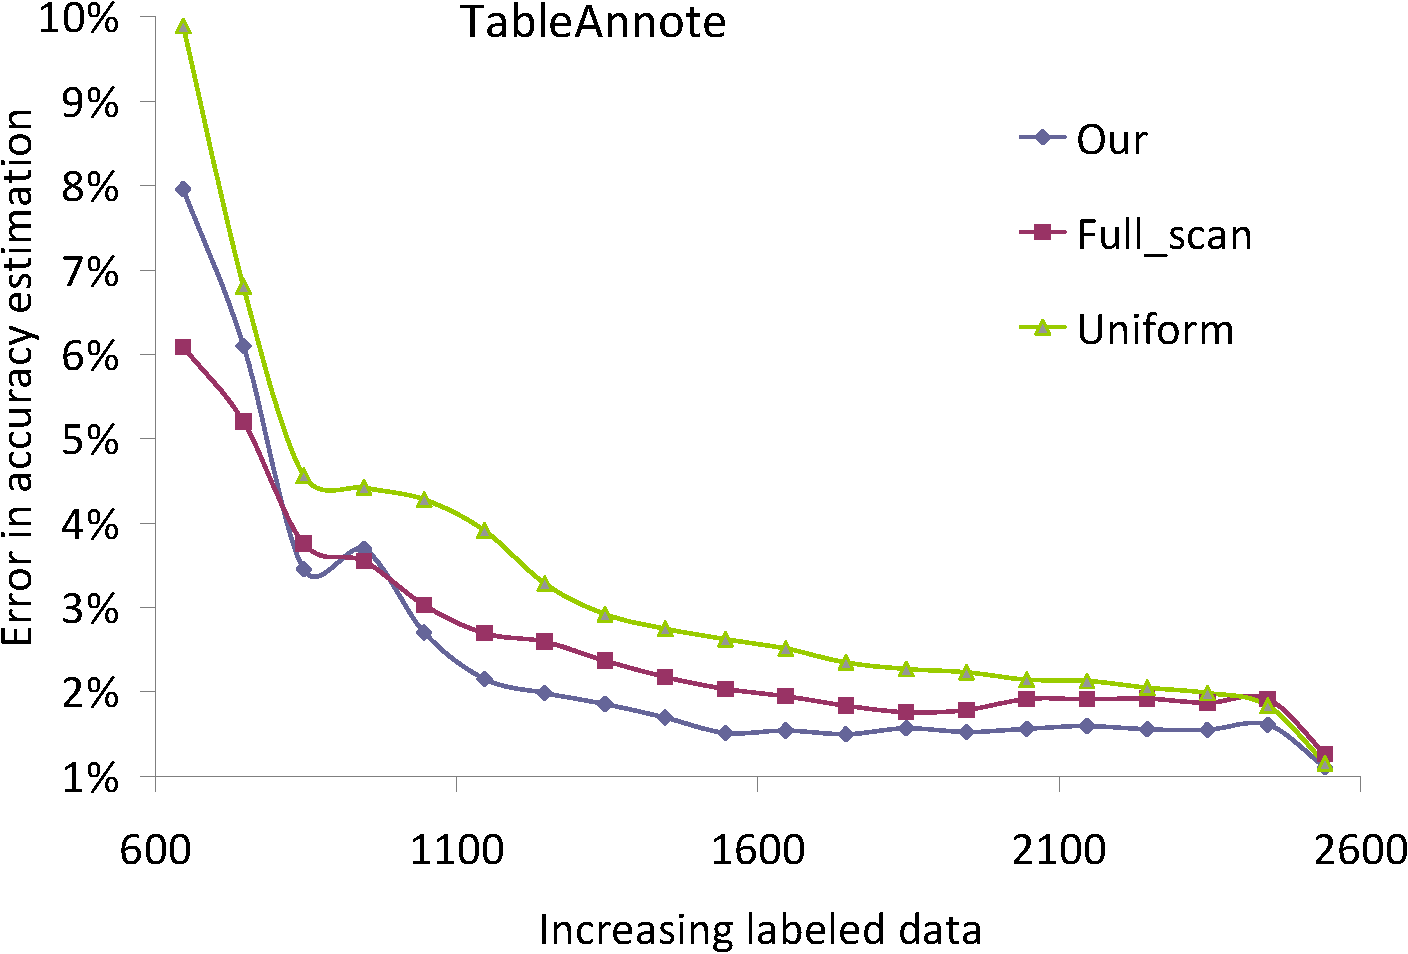
\includegraphics[width=0.30\hsize]{figs/selectB5-crop}
%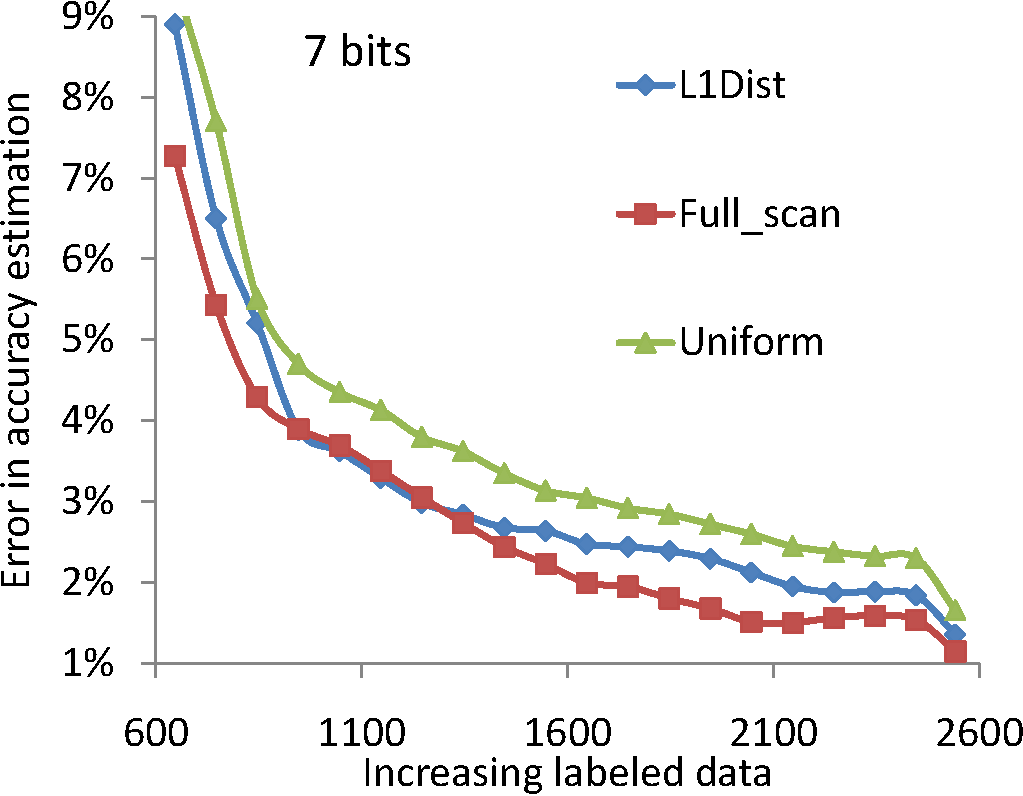
\includegraphics[width=0.30\hsize]{figs/selectB7-crop}
%\end{center}
%\end{frame}
%
%%%%%%%%%%%%%%%%%%%%%%%%%%%%%%%%%%%%%%%%%%%%%%%%%%%%%%%%%%%%%%%%%%%%%%%
%
%\section{Conclusions}
%\begin{frame}
%\frametitle{Conclusions}
%\begin{center}
%\begin{itemize}
%\item Proposed method of estimating the accuracy of a
%classifier on very large and diverse dataset  
%\item Method based on stratified sampling theory and makes following contributions beyond existing
%methods 
%\begin{itemize}
%\item Develop a stratification method based on $r$ bit
%signatures learned using a novel signed logistic algorithm
%\item Perform stratified sampling directly on indexed
%unlabeled data without requiring full data scan on every data
%re-stratification
%\end{itemize}
%\item Experiments on several real datasets show that our method provides
%more accurate estimates than existing methods, and that our strategies
%for accessing unlabeled data gives close to optimal performance while
%reading orders of magnitude fewer instances.
%\end{itemize}
%\end{center}
%\end{frame}